\documentclass[10pt]{article}
\usepackage[margin=0.9in]{geometry}
\usepackage{graphicx}
\usepackage{booktabs}
\usepackage{amsmath}
\usepackage{hyperref}
\usepackage{caption}
\usepackage{float}
\captionsetup{font=small}
\usepackage{enumitem}
\setlist{nosep}

\title{\bf Small Language Models at the Solar Edge: \\
An Empirical Survey of Function Calling, Hybrid Architectures, \\
and Speculative Decoding on an 8\,GB Jetson}
\author{Walker Kirkpatrick \\
\small Generated with the Hermes agent; all measurements from the author's device}
\date{October 1, 2026}

\begin{document}
\maketitle

\begin{abstract}
We report a series of empirical benchmarks of small language models (SLMs)
on a Jetson Orin Nano 8\,GB development kit operating from a 100\,W solar
panel with battery buffer, chosen as a representative energy-constrained
edge platform with 68\,GB/s shared memory bandwidth.\,[5] Across three
campaigns we measure: (1) function-calling accuracy of 17 open models on a
52-test BFCL-style suite, where the hybrid Mamba2 model Granite 4.0-3B
scored 96.2\% and was the only sub-4B model to pass chained tool calls
(7/8); (2) context-window and KV-cache quantization ceilings for the same
model, mapping a four-profile operating envelope from 32K f16 to the full
131K native window at q4\_0; and (3) decode/prefill speeds of six current
3B-class models plus one 8B model on llama.cpp 0.5.0-dev, where the hybrid
conv+GQA model LFM2.5-VL-3B with a DSpark speculative drafter achieved
34--37 tok/s --- the fastest decode measured on this hardware, a
$1.4\times$ speedup over its own non-drafted baseline. We find that hybrid
attention architectures dominate the accuracy--speed--memory trade-off at
this scale: they concentrate KV cache into a few attention layers, enabling
both long context and fast decode, and we show a dense 8B model cannot
achieve even 42K context on this hardware at any quantization. We release
all launch settings, raw results, and the PDF in the companion repository.
\end{abstract}

\section{Introduction}
Edge inference of language models is increasingly practical: 3B-class
models now fit in under 2\,GB as 4-bit GGUF quants, and open runtimes such
as llama.cpp provide an OpenAI-compatible server on Arm+CUDA
hardware.\,[8] This paper consolidates three benchmark campaigns executed
between September and October 2026 on a single Jetson Orin Nano 8\,GB
(Ampere GPU, 1024 CUDA cores, 8\,GB LPDDR5 shared between CPU and GPU,
68\,GB/s stock memory bandwidth).\,[5] The device runs headless (display
manager disabled) to free $\sim$1.5\,GB of RAM, and is solar-powered via a
100\,W panel and battery buffer drawing a net 11.30\,W under inference
load.

The campaigns answer three questions a practitioner faces when deploying a
local agent stack:
\begin{enumerate}
\item \textbf{Which small model calls tools most reliably?} (\S\ref{sec:bfcl})
\item \textbf{How much context can the winner actually use under real memory pressure?} (\S\ref{sec:context})
\item \textbf{What is the current speed frontier, and does speculative decoding pay off?} (\S\ref{sec:speed})
\end{enumerate}
All numbers are measured on-device; nothing is taken from vendor
literature. Where an external fact is cited (architecture details, hardware
specifications, method definitions), it is marked with a numbered
reference.

\section{Method}
\label{sec:method}
\textbf{Hardware.} Jetson Orin Nano 8\,GB developer kit, JetPack 6.x with
CUDA 12.6, GDM disabled during benchmarks. We set
\texttt{GGML\_CUDA\_ENABLE\_UNIFIED\_MEMORY=1} for all runs, which allows
KV-cache and compute-buffer allocation into the shared memory space.

\textbf{Engine.} llama.cpp v0.5.0-dev, build 965 (commit \texttt{ec7630a}),
compiled with \texttt{CMAKE\_CUDA\_ARCHITECTURES=87}; an earlier campaign
used build 794 (commit \texttt{84e76d8}).\,[8]

\textbf{Function-calling evaluation.} A 52-test BFCL-style suite spanning
four categories: 30 simple calls, 12 moderate parallel calls, 8 moderate
chained (two-step) calls, and 2 coding tasks, executed against a local
OpenAI-compatible server with greedy decoding (temperature 0.0) per the
model vendor's tool-calling guidance. The Berkeley Function Calling
Leaderboard (BFCL) is the reference executable benchmark for this
capability; its categories evaluate AST-level call correctness, parallel
dispatch, and multi-step chaining.\,[6][7]

\textbf{Speed measurement.} Wall-clock completion of fixed prompts
(300-token generations for decode speed; 7.4--29.9K-token prompts for
prefill) via the \texttt{/v1/chat/completions} endpoint, three runs each.
Reasoning/thinking modes were disabled per-model (either soft switches or
template kwargs) so that decode speed reflects useful output tokens.

\textbf{Architectural decode.} Model internals (layer counts, KV-head
layouts, context lengths, chat-template switches) were decoded directly
from each GGUF's metadata fields rather than assumed from model cards.

\section{Results I: Function-calling accuracy}
\label{sec:bfcl}

\begin{figure}[H]
\centering
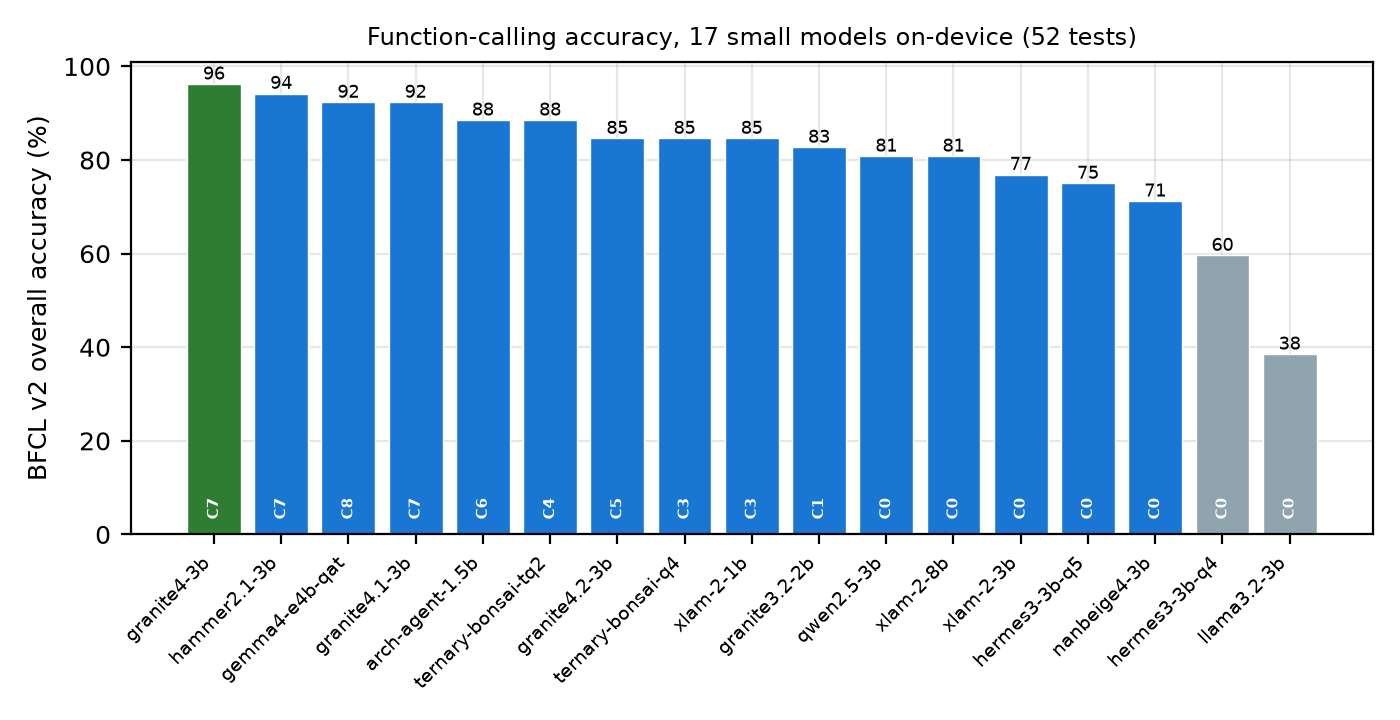
\includegraphics[width=\linewidth]{../results/figures/fig1_bfcl.png}
\caption{BFCL-style overall accuracy, 17 models, 52 tests each. White
bars inside columns (C$n$) show chained-call passes out of 8. Granite
4.0-3B (green) leads at 96.2\%.}
\end{figure}

The full ranking appears in Fig.~1. Three findings stand out:

\begin{enumerate}
\item \textbf{Granite 4.0-3B leads at 96.2\%} (50/52), including 7/8
chained calls and 12/12 parallel calls. Its hybrid Mamba2 architecture
places only four full-attention layers among 40 total blocks.\,[9] The
same vendor's dense successor models score lower on this suite
(Granite 4.1-3B and Granite 4.2-3B at 92.3\% and 84.6\%), suggesting
generation upgrades do not automatically transfer tool reliability.
\item \textbf{Chained calls are the separator.} Nine of seventeen models
scored zero on chained (two-step) tool calls while often passing simple
single calls at high rates --- e.g., Qwen2.5-3B scored 80.8\% overall but
0/8 chained. Only five models passed at least half the chained tests.
\item \textbf{Size alone does not rescue function calling.} The 8B
xLAM-2-8B (80.8\%) did not beat several 3B models, and the 1.5B
Arch-Agent scored 88.5\% --- outperforming half the 3B field.
\end{enumerate}

\section{Results II: Context and KV-quantization ceilings}
\label{sec:context}

Granite 4.0-3B advertises a 131K native window. Realizing it on 8\,GB
shared memory requires quantizing the KV cache itself. We measured
load/generate viability for every combination of context length and KV
quantization, with the model fully offloaded (\texttt{-ngl 99}); on this
llama.cpp build the hybrid's KV cache then resides on GPU.\footnote{On
older builds with partial offload, KV fell back to host memory with a
$\sim$3$\times$ decode penalty; the \texttt{-ngl 99} full-offload finding
supersedes earlier partial-offload guidance for hybrid SSM models on
current builds.}

\begin{figure}[H]
\centering
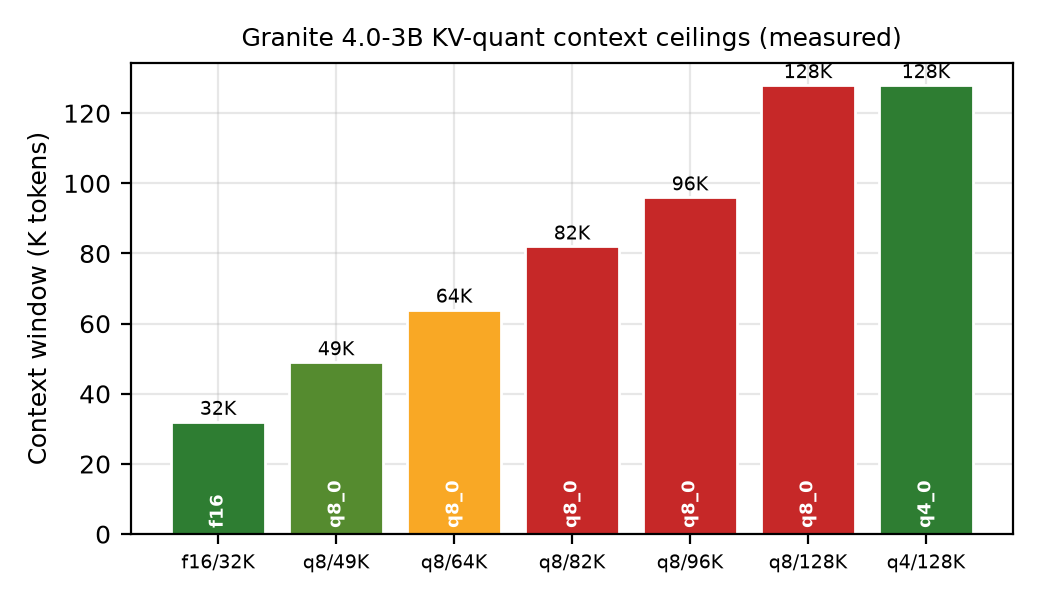
\includegraphics[width=0.78\linewidth]{../results/figures/fig5_kv_ceilings.png}
\caption{Measured context ceilings by KV type. Green: usable. Yellow:
standalone only. Red: allocation failure. q4\_0 KV is the only path to
the full 131K window.}
\end{figure}

\begin{figure}[H]
\centering
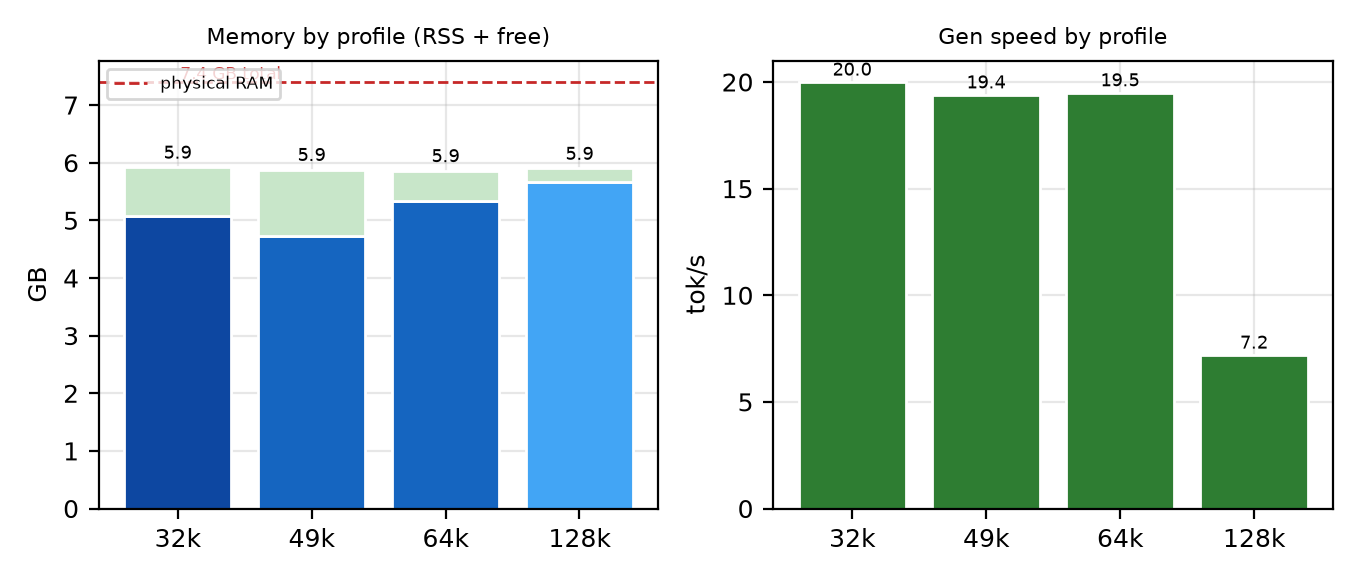
\includegraphics[width=\linewidth]{../results/figures/fig4_granite_profiles.png}
\caption{The four operating profiles: memory footprint (left) and decode
speed (right). The 49K profile is the agent-safe default; 64K OOM-dies
under a full KV plus concurrent gateway load; 128K trades decode speed
(7.2 tok/s at depth) for full window.}
\end{figure}

The resulting operating envelope is four profiles: 32K/f16 (20.0 tok/s),
49K/q8\_0 (19.4 tok/s, 1.16\,GB free --- the only profile that survives a
full KV plus a resident agent gateway), 64K/q8\_0 (19.5 tok/s, standalone
only), and 128K/q4\_0 (7.2 tok/s at 29K depth, 5.66\,GB RSS). Failed
configurations died in two distinct modes: compute-buffer allocation
failures at load (82K/96K/128K q8\_0), and --- more subtly --- a kernel
OOM kill of a successfully loaded 64K server when a deep generation filled
the KV and the agent gateway's request landed on top. The lesson: a
launch-time memory check is necessary but not sufficient; the envelope
must be drawn against \emph{runtime} KV fill, not just load footprint.

\section{Results III: The speed frontier and speculative decoding}
\label{sec:speed}

\begin{figure}[H]
\centering
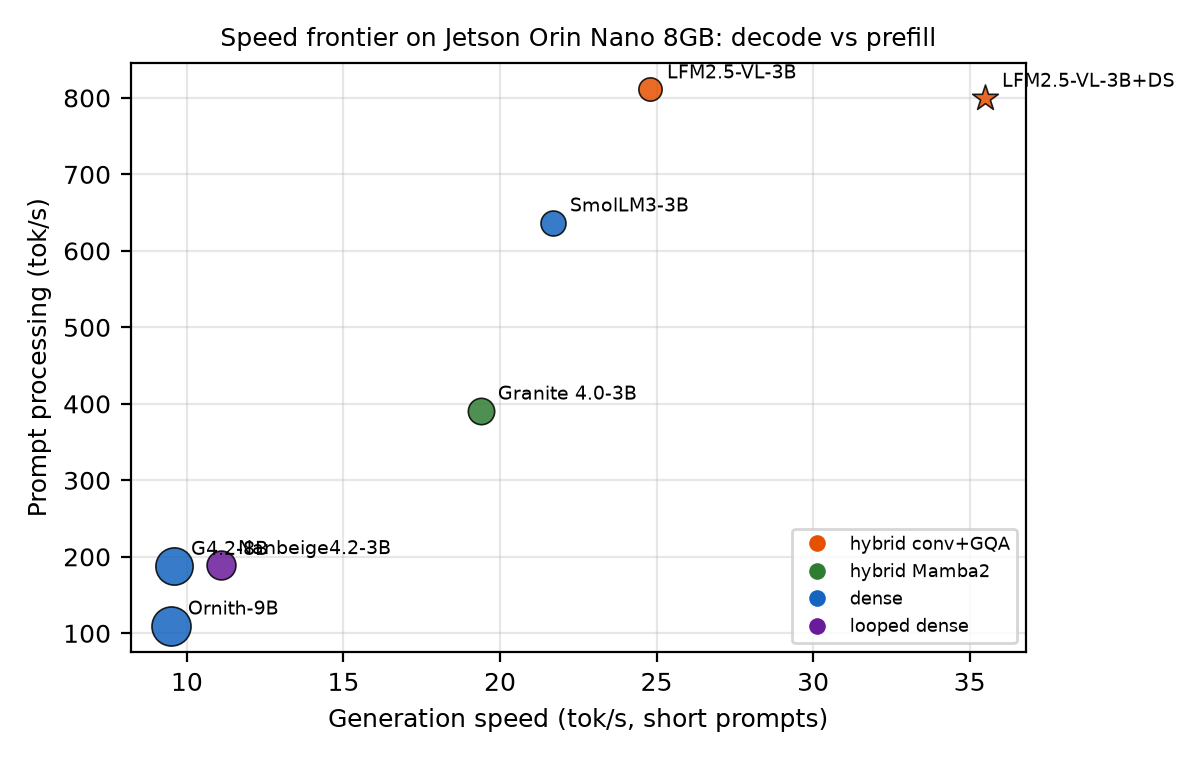
\includegraphics[width=0.85\linewidth]{../results/figures/fig2_speed_frontier.png}
\caption{Decode vs prefill for seven models. Marker area $\propto$ GGUF
file size; color = architecture. LFM2.5-VL-3B+DSpark defines the
frontier.}
\end{figure}

\begin{table}[H]
\centering
\small
\begin{tabular}{lrrrrl}
\toprule
Model & tok/s & pp t/s & Arch & GB & Tool calls \\
\midrule
\textbf{LFM2.5-VL-3B + DSpark} & \textbf{34--37} & 787--811 & hybrid & 2.09 & native \\
LFM2.5-VL-3B & 24.5--25.1 & 811 & hybrid & 1.56 & native \\
SmolLM3-3B & 21.4--22.1 & 637 & dense & 1.80 & parse gap \\
Granite 4.0-3B & 19.4 & 391 & hybrid & 2.00 & native \\
Nanbeige4.2-3B & 11.0--11.2 & 189 & looped & 2.40 & native \\
Granite 4.2-8B IQ3\_M & 9.6 & 188 & dense & 4.00 & kwarg \\
Ornith-1.0-9B IQ3\_M & 9.5 & 110 & dense & 4.40 & --- \\
\bottomrule
\end{tabular}
\caption{Speed frontier, short-prompt decode and 7.4K prefill, llama.cpp
build 965. Tool calls: native = standard \texttt{tool\_calls} object;
parse gap = correct JSON emitted inside fenced content but not parsed;
kwarg = requires \texttt{enable\_thinking:false} template kwarg.}
\end{table}

\textbf{Speculative decoding with DSpark.} The LFM2.5-VL-3B DSpark
drafter is a $\sim$280M-parameter companion that reads the target's
hidden states to propose up to $k$ tokens ahead, verified in one target
forward pass; it ships with day-one llama.cpp support.\,[1][2][12] On
this hardware with $n_{\max}{=}3$, acceptance rates measured 38--50\% on
prose and 100\% on a greedy tool-call turn, yielding 34--37 tok/s versus
24.5--25.1 tok/s for the target alone --- a $1.43\times$ speedup, at the
cost of 0.53\,GB extra file and negligible latency (Fig.~3). Prefill is
unaffected, as expected for decode-only speculation. Vendor-reported
gains on larger hardware reach $2.1\times$ (llama.cpp, M3 Ultra) with
task-dependent acceptance.\,[1] The headroom between our 38--50\% and
their higher acceptance suggests larger draft budgets ($n_{\max} > 3$)
may pay off on this hardware too; this is future work.

\begin{figure}[H]
\centering
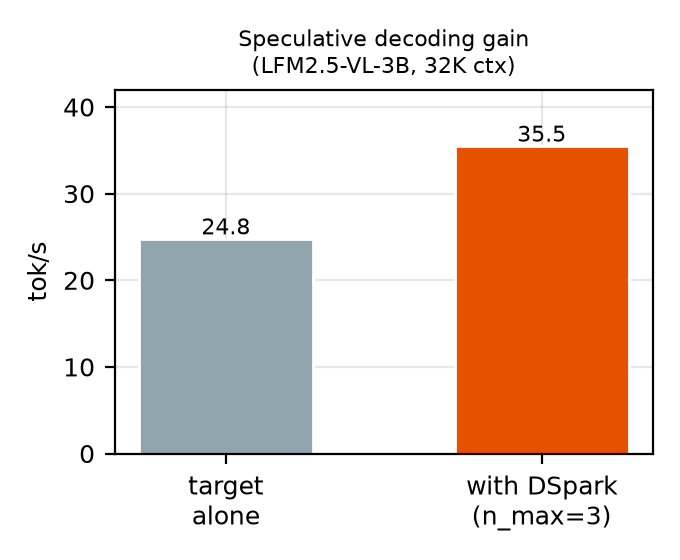
\includegraphics[width=0.45\linewidth]{../results/figures/fig3_dspark_gain.png}
\caption{DSpark speculative decoding: 24.8 to 35.5 tok/s ($1.4\times$),
identical prefill.}
\end{figure}

\textbf{Looped transformers pay a compute tax.} Nanbeige4.2-3B feeds its
hidden states through the same 22-layer stack twice, increasing effective
depth without extra parameters.\,[3][10] The model card credits this loop
with outperforming larger models on agentic benchmarks; on our hardware
the doubled forward passes halve decode speed relative to the hybrid
conv+GQA frontier (11.1 vs 25--37 tok/s), consistent with an independent
Apple-Silicon deployment study that optimized precisely this looped-model
memory/compute overhead.\,[4] Its 262K advertised window is unreachable
on 8\,GB at any KV quantization (dense 88\,KB/token KV).

\textbf{Dense 8B cannot reach 42K context here.} Granite 4.2-8B is a
40-layer dense model with 160\,KB/token f16 KV --- 6.9\,GB of KV alone at
42K, exceeding the machine. Even IQ3\_M weights (4.0\,GB) with q4\_0 KV
reach only 16K with 1.03\,GB headroom, decoding at 9.6 tok/s. The model's
agentic RL training is real, but on this hardware the dense architecture
is strictly dominated by the 3B hybrids.

\textbf{Engine upgrade does not change SSM decode.} Rebuilding llama.cpp
from build 794 to 965 (171 commits, including CUDA convolution
acceleration) left Granite 4.0-3B decode within noise (19.3--19.6 vs 19.5
tok/s) and improved prefill at 29K depth by 8\% (391 vs 362 t/s): the new
conv work targets conv2d/3d vision kernels, not the conv1d path used by
Mamba2 hybrids.

\section{Cross-cutting findings}

\begin{enumerate}
\item \textbf{Hybrid attention models dominate this tier.} The two
hybrid architectures tested (Mamba2, conv+GQA) own the top of every axis:
accuracy (96.2\%), decode speed (35 tok/s), context (131K), and memory
efficiency. Concentrating KV into few attention layers is the mechanism
--- the dense 8B comparison makes the causal effect visible at fixed
capability.
\item \textbf{Tool-call reliability and raw speed are different axes.}
The BFCL champion (Granite 4.0-3B, 19.4 tok/s) is not the speed
champion (LFM2.5-VL-3B+DSpark, 37 tok/s, untested on BFCL here), and
neither is the chat-quality leader. Agent stacks should pick per role.
\item \textbf{Thinking defaults are a deployment trap.} Two models
defaulted to reasoning mode and silently burned entire token budgets in
\texttt{reasoning\_content} with empty visible output; both need explicit
off-switches (template kwarg for Granite 4.2, Qwen-style \texttt{think}
soft switch for LFM2.5). A related earlier finding: a thinking-required
successor model (Ornith-1.5-9B) \emph{underperformed} its non-thinking
predecessor on long generations because required thinking loops
dominated short context budgets.
\item \textbf{Launch method matters on memory-capped boards.} Processes
launched inside a systemd worker scope with a $\sim$5\,GB memory ceiling
were OOM-killed mid-load despite free system RAM; escaping the scope
(\texttt{setsid}) is part of our required launch settings, as is
disabling the display manager ($\sim$1.5\,GB reclaimed).
\end{enumerate}

\section{Limitations}
Scores are from a single 52-test suite rather than the full live BFCL
(5{,}088 items in v4); absolute percentages would shift on the full
benchmark, though the separation on chained calls is stark and consistent
with the leaderboard's own finding that multi-step tool use is the
hardest category.\,[6] Speeds are wall-clock averages of three runs, not
paired statistical tests. The solar figure (11.30\,W net under load)
comes from a separate energy campaign and is quoted, not re-measured
here. Acceptance rates for DSpark were read from engine logs at default
$n_{\max}{=}3$; tuning is future work.

\section{Conclusions}
On an 8\,GB edge device, hybrid-attention 3B models are the only class
that simultaneously delivers top function-calling accuracy, the full
native context window, and the fastest decode --- with speculative
decoding extending the lead to 34--37 tok/s. Dense models, including a
newer and nominally more capable 8B, cannot compete for context on this
memory budget, and looped architectures trade decode speed for depth at
a rate this hardware cannot afford. The recommended local agent stack on
this box: LFM2.5-VL-3B with DSpark for speed-critical chat, Granite
4.0-3B at the 49K profile for reliable tool calling, both served by
llama.cpp build 965+ under \texttt{setsid} with the display manager off.

\section*{Sources}
\small
\begin{enumerate}
\item \url{https://www.liquid.ai/blog/lfm2-5-vl-dspark} — LFM2.5-VL-DSpark announcement (acceleration figures, llama.cpp day-one support).
\item \url{https://arxiv.org/abs/2607.05147} — Cheng et al., DSpark: Confidence-Scheduled Speculative Decoding with Semi-Autoregressive Generation.
\item \url{https://arxiv.org/pdf/2607.22083} — Nanbeige4.2-3B: Unlocking Agentic Capabilities in a Compact Model.
\item \url{https://arxiv.org/html/2608.13987v1} — Halloran, Nanbeige4.2-3B on Apple Silicon (looped-transformer overhead).
\item \url{https://www.nvidia.com/en-us/autonomous-machines/embedded-systems/jetson-orin/nano-super-developer-kit} — Jetson Orin Nano Super specs (1024 CUDA cores, 68 GB/s stock bandwidth).
\item \url{https://gorilla.cs.berkeley.edu/leaderboard.html} — BFCL V4 leaderboard (category structure; multi-step as hardest category).
\item \url{https://github.com/ShishirPatil/gorilla/blob/main/berkeley-function-call-leaderboard/bfcl_eval/data/README.md} — BFCL dataset categories.
\item \url{https://github.com/ggml-org/llama.cpp} — llama.cpp inference engine.
\item \url{https://arxiv.org/html/2609.35378v1} — Multilinguality in Hybrid Attention LLMs (Granite-4.0-H: 4 attention layers of 40).
\item \url{https://huggingface.co/Nanbeige/Nanbeige4.2-3B-Base} — model card (looped architecture, 28T tokens).
\item \url{https://recipes.vllm.ai/LiquidAI/LFM2.5-350M} — LFM2.5 hybrid backbone description (conv + GQA).
\item \url{https://www.liquid.ai/blog/lfm2.5-dspark} — LFM2.5-DSpark draft checkpoints (mechanism, llama.cpp support).
\end{enumerate}

\end{document}